% Overrides original definition
\def\rmhtmet{\mbox{$\mathcal{R}$}\xspace}

%%____________________________________________________________________________||
\newpage
\section{QCD multijet background estimation\label{sec:qcd}}

One of the major challenges for searches of new physics in the jets +
\met final state is the control of background events from QCD multijet
production. The difficulties in the determination of precise estimates
for this background stem from the large cross sections expected at the
LHC, compounded by the lack of precise theoretical predictions for
these cross sections and the kinematic properties of multijet
events. Hence, without special consideration and treatment,
significant uncertainties on large background expectations can
overwhelm any potential sensitivity to new physics signatures.

With regards to QCD multijet production, the approach of this search
is to favour the suppression of the multijet background to a
negligible level. A conservative uncertainty on a negligible
contribution is preferred over a procedure that attempts to accurately
estimate a non-negligible contribution from multijet events. The level
of contamination should be sufficiently small (\ie percent level) such
that the associated uncertainty, even if large, will be subdominant
with respect to the uncertainties on the remaining SM backgrounds with
genuine \met, such as \wj, \ttbar, and \znunu.

Hence, the signal region is defined in a manner that suppresses the
expected contribution from multijet production to a low (\ie percent)
level with respect to the total expected background from other SM
processes for all signal region bins. This is achieved primarily
through the application of very tight requirements on the variables
\alphat, \bdphi, and $\mhtmet$, as described in
Section~\ref{sec:had-signal}. 

The \alphat variable, described in Section~\ref{sec:alphatdef}, is
able to distinguish with high efficiency the sources of ``fake'' \met,
such as jet energy mismeasurement, from those with ``genuine'' \met,
such as neutrinos.  The \bdphi variable, described in
Section~\ref{sec:bdphi-def}, is also very efficient at identifying
jets that suffer under-measurements, as well as over-measurements, in
multijet events. The variable is also particularly suited to
identifying multijet events that exhibit significant \met due to the
production of neutrinos, collinear with a jet axis, in semileptonic
heavy-flavour decays. Both variables are individually capable of
reducing the yields from multijet events by several orders of
magnitude, and combined provide an extremely robust method to reject
multijet events. Figure~\ref{fig:alphat_bdphi_distr} shows the
distributions in data for the \alphat and \bdphi variables. The
$\mht/\met$ variable, described in Sec.~\ref{sec:mhtmet}, further
suppresses the QCD multijet background due to events containing
multiple jets outside the experimental acceptance that contribute
significantly to \mht.

\begin{figure}[!h]
 \centering
 \subfigure[\alphat distribution.\label{fig:alphat_distr}]{
 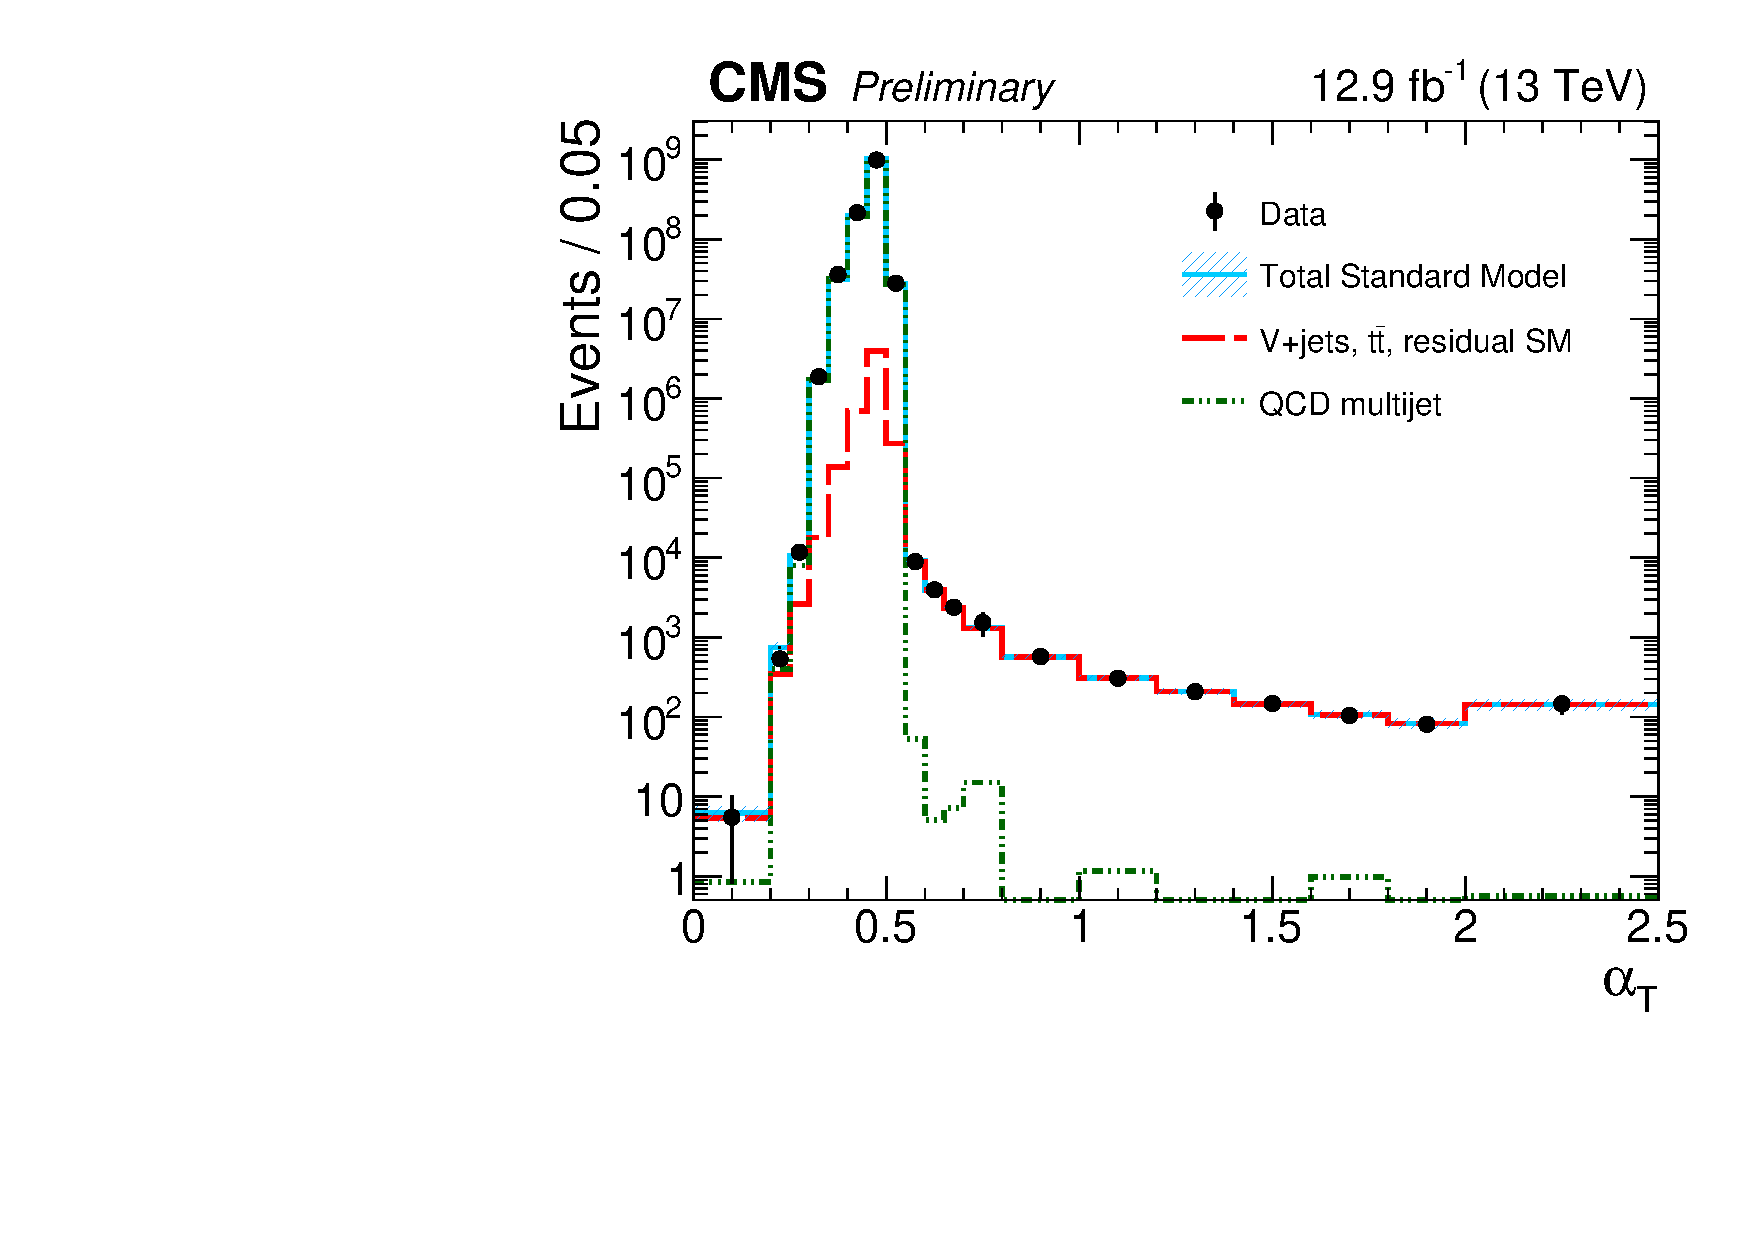
\includegraphics[width=0.5\textwidth]{figures/qcd/CMS-PAS-SUS-16-016_Figure-aux_001.pdf}
 }
 \subfigure[\dphimhtj distribution.\label{fig:bdphi_distr}]{
 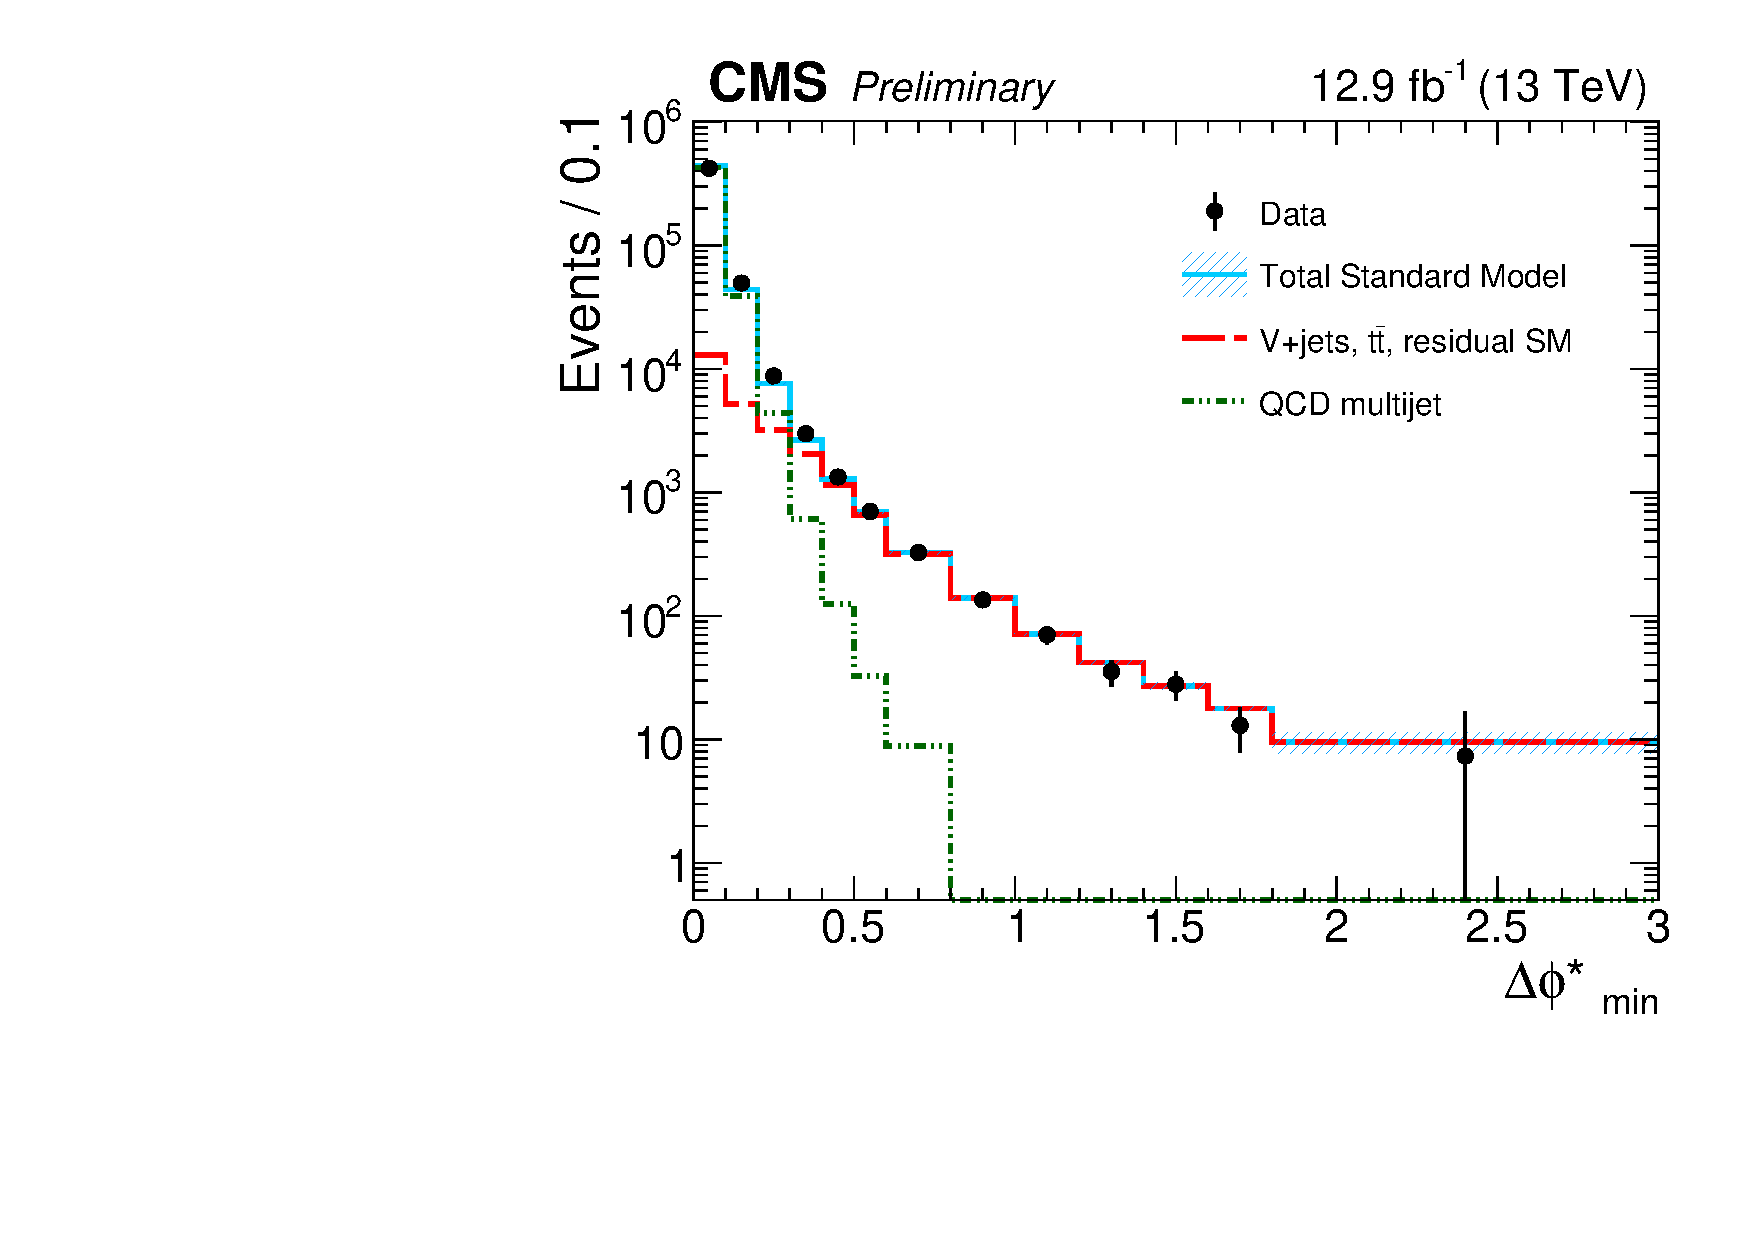
\includegraphics[width=0.5\textwidth]{figures/qcd/CMS-PAS-SUS-16-016_Figure-aux_002.pdf}
 } \\
 \caption{(Left) The \alphat distribution in data for events
   satisfying the pre-selection criteria when $\alphat < 0.55$ and the
   full signal selection criteria when $\alphat > 0.55$. (Right) The
   \bdphi distribution in data for events satisfying the pre-selection
   criteria and $\scalht > 800\GeV$. }%\fixme{UPDATE!} 
 \label{fig:alphat_bdphi_distr}
\end{figure}

\subsection{Overview of the method}
\label{sec:qcdMethod}

An estimate of the QCD multijet background is determined using three
multijet-enriched data sidebands, defined by inverting one or both
signal-region requirements on \bdphi and
$\mht/\met$. Table~\ref{tab:qcd_sidebands} summarises the requirements
for the three sideband regions and the signal region, labelled
\textbf{A}, \textbf{B}, \textbf{C}, and \textbf{D},
respectively. Further details on the selection requirements can be
found in Sec.~\ref{sec:multijetcontrolSelection}. The triggers used to
record the event samples are described in
Sec.~\ref{sec:control_samples}. A study of the correlation between
\bdphi and $\mht/\met$, per $(\njet, \scalht)$ category, is shown in
Tab.~\ref{tab:bdphi_mhtmet_correlation} (Appendix~\ref{app:qcd}). A
low level of correlation was found between the two variables since the
\bdphi variable identifies multijet events characterised by
significant ``fake'' \met due to the mismeasurement of jets within the
experimental acceptance, while $\mht/\met$ identifies events
characterised by significant ``fake'' \met due to the presence of jets
outside the experimental acceptance that contribute to \mht. 

\begin{table}[h!]
  \caption{Definitions of data sidebands used in the determination of
    the QCD multijet background in the signal region. }  
  \label{tab:qcd_sidebands}
  \centering
  \footnotesize
  \begin{tabular}{ r|l|l }
                           & \multicolumn{1}{c|}{$0.2 < \bdphi < 0.5$} & \multicolumn{1}{c}{$\bdphi > 0.5$} \\[0.8ex]
    \hline
    $1.25 < \mhtmet < 3.0$ & \textbf{A} (``Double sideband'')         & \textbf{B} (``\mhtmet sideband'')  \\[0.8ex]
    \hline
    $\mhtmet < 1.25$       & \textbf{C} (``\bdphi sideband'')         & \textbf{D} (``Signal region'')     \\[0.8ex]
  \end{tabular}
\end{table}

The background estimation is performed in (\njet, \scalht) bins in
each of the data sidebands. The \njet and \scalht distributions in
each of the sidebands can be found in
Figs.~\ref{fig:qcd_distributions_1}~and~\ref{fig:qcd_distributions_2}.
The observed counts in each $(\njet, \scalht)$ are corrected to
account for contamination from non-multijet SM processes. The
corrected counts $\mathcal{N}_i^\text{data}(\njet, \scalht)$ are
assumed to arise solely from QCD multijet production. The subscript
$i$ indicates the sideband under consideration (\textbf{A},
\textbf{B}, or \textbf{C}). The non-multijet processes, which comprise
vector boson and \ttbar production and residual contributions from
other SM processes, are estimated using corresponding sidebands to the
\mj and \mmj control regions, as described in Secs.~\ref{sec:ttw} and
\ref{sec:zinv}, respectively.

Independent ratios $\mathcal{R}_i^\mathrm{QCD}(\njet, \scalht)$ of the
number of multijet events that satisfy one or both of the
signal-region requirements to the number that fail the same
requirements are determined from simulation for events categorised
according to \njet and \scalht, and inclusively with respect to \nb
and \HTmiss. The subscript $i$ for each ratio $\mathcal{R}_i$
indicates the sideband (\textbf{A}, \textbf{B}, or \textbf{C}) from
which the extrapolation is being performed. The product of each ratio
$\mathcal{R}_i^\mathrm{QCD}(\njet, \scalht)$ and the corresponding
corrected data count $\mathcal{N}_i^\text{data}(\njet, \scalht)$
provides the estimate of the multijet background $\mathcal{P}_i(\njet,
\scalht)$. 

The estimates as a function of \njet, \scalht, \nb, and \HTmiss of the
signal region are assumed to factorise as follows:
\begin{equation}
  \label{eq:qcd1}
  \mathcal{P}_i( \njet, \scalht )  =
  \mathcal{N}_i^\text{data}( \njet, \scalht )\;
  \mathcal{R}_i^\mathrm{QCD}( \njet, \scalht ),
\end{equation}
\begin{equation}
  \label{eq:qcd2}
  \mathcal{P}_i( \njet, \scalht, \nb, \HTmiss ) = 
  \mathcal{P}_i( \njet, \scalht )\;
  \mathcal{K}_{\njet, \scalht}( \nb, \HTmiss ), 
\end{equation}
where the subscript $i$ refers to the sideband (\textbf{A},
\textbf{B}, or \textbf{C}). 

The $\mathcal{K}_{\njet, \scalht}( \nb, \HTmiss )$ are multiplier
terms that provide the estimated distribution of events as a function
of \nb and \HTmiss while preserving the normalisation $\mathcal{P}_i(
\njet, \scalht )$. The distribution of multijet events as a functions
of \nb and \HTmiss, $\mathcal{K}_{\njet, \scalht}( \nb, \HTmiss )$, for
the multijet and non-multijet backgrounds are compared in 
Figs.~\ref{fig:qcd_nb_shapes_mhtmetsb}~to~\ref{fig:qcd_mht_shapes_doublesb}.
Although the multijet components falloff faster than the non-multijet
components with increasing \nb or \HTmiss, the within the applied
systematic uncertainty, the multijet and non-multijet $(\nb, \HTmiss)$
shapes are consistent. Hence, the non-multijet shape is used for the
multijet prediction due to the higher MC statistics.

\subsection{Binned maximum-likelihood approach}
%estimate per \texorpdfstring{(\njet, \scalht)}{(Njet, HT)} bin}
% for \texorpdfstring{$\mathcal{P}_i( \njet, \scalht )$}{P(Njet,HT)}}

In this section, the multijet process is henceforth labelled as
``QCD''. The non-multijet processes (primarily \wj, \ttbar, and
\znunu) are henceforth labelled as collectively as the ``EWK''
processes.

A binned maximum-likelihood (ML) fit to data counts in each sideband,
analagous to that described in Sec.~\ref{sec:likelihood}, is performed
to obtain an estimate of the number of QCD multijet events in each
(\njet, \scalht) bin of a given sideband region. The EWK contributions
in the data sidebands are estimated using the ``transfer factor''
method, described in Secs.~\ref{sec:tf-method-ttw} and
\ref{sec:tf-method-zinv}, and the \mj and \mmj control regions,
defined by the same selection criteria described in
Sec.~\ref{sec:control-region-selection} except for the inverted
requirement on the sideband variables. The fit to data assumes only
the presence of QCD and EWK contributions. Signal contamination is
expected to be negligible. All relevant systematic uncertainties in
the EWK background estimates are taken into account, including the
sources of experimental uncertainties described in
Secs.~\ref{sec:systematics}
and~\ref{sec:systematics-zinv}. Independent fits are performed per
sideband region.

The fit for each sideband region is used to constrain a free parameter
$\mu_{\textrm{QCD}}$ per (\njet, \scalht) bin that acts as a
multiplier term on the nominal QCD expection per bin, as determined
from simulation. The ML value of the (``signal strength'')
$\mu_{\textrm{QCD}}$ parameter per bin is applied to the nominal QCD
expectation (from simulation) in the corresponding bin of the signal
region to give an estimate for the QCD background. The three
independent fits therefore provide three independent predictions per
(\njet, \scalht) bin.

Figures~\ref{fig:mhtmet_sideband} (see Appendix~\ref{app:qcd})
summarises the following information obtained from the fit in the
$\mhtmet$ sideband: the observed data counts, the post-fit estimates
of the both the EWK and QCD contributions, and the constrained values
of the floating parameters $\mu_{\textrm{QCD}}$, as a function of
\njet and \scalht for the each of the sidebands. The pre-fit QCD
expectations are shown, but these can be inferred from the post-fit
expectations and ML values of $\mu_{\textrm{QCD}}$. Similarly, the
same information is shown for the \bdphi and ``double'' sidebands in
Figs~\ref{fig:bdphi_sideband} and~\ref{fig:double_sideband} (both in
Appendix~\ref{app:qcd}), respectively.

The QCD background estimate for each (\njet, \scalht) bin in the
signal region is determined from a weighted average of the predictions
based on each of the three sideband regions. 
%\footnote{In the case of zero QCD expectation in any given signal
%  region bin due to finite-size simulated event samples, the
%  uncertainty is estimated from neighouring bins.}
%the error is estimated by taking a poisson error with the average
%weight of QCD events in that bin before any analysis selection is
%applied.
%This takes advantage of the fact that different sidebands typically
%populate different ares of the \njet and \scalht phase space.  
Figure~\ref{fig:qcd_estimate} (Appendix~\ref{app:qcd}) shows the
(weighted) expected QCD background per (\njet, \scalht) bin, as
determined from the procedure above, and the expected EWK background
per bin in the signal region, as determined from the methods described
in Secs.~\ref{sec:ttw} and~\ref{sec:zinv}. Finally, the ratio of the
QCD and EWK background expectations per bin is also shown. The QCD
background is estimated to be negligible with respect to the EWK
background, typically below the percent level. This level of
contamination is compatible with the levels seen for pervious
iterations of this search, at both $\sqrt{s} = 8$ and 13\TeV. The
predicted multijet event counts are included as a background
contribution to the likelihood model, described in
Sec~\ref{sec:likelihood}.

\subsection{Validation of the model and systematic uncertainties}
\label{sec:qcdValidation}

The reliance on simulation to model correctly the extrapolation from
each data sideband via the ratios $\mathcal{R}_i^\mathrm{QCD}$ is
validated by comparing the independent estimates $\mathcal{P}_i(\njet,
\scalht)$ from each sideband region. The level of closure in the
method is determed by comparing the differences in the ML values of
$\mu_{\textrm{QCD}}$ determined from each sideband region. The ML
values for $\mu_{\textrm{QCD}}$ determined from the \mhtmet and \bdphi
sideband regions are shown relative to the those obtained from the
``double'' sideband, the largest and purist event sample, in
Fig.~\ref{fig:qcdVal} (Appendix~\ref{app:qcd}). Bins for which there
are insufficient event counts in data or simulation to make the
calculation are not shown. Good agreement between the estimates
indicates a good control over the simulation modelling and the
determination of EWK contamination and trigger efficiencies in each of
the sideband regions. An adequate level of agreement between the
independent predictions is observed, and is amply covered by an
assumed systematic uncertainty of 100\% in each (weighted)
estimate. This uncertainty is assume to be unccorrelated across
(\njet, \scalht) bins.

The distribution of multijet events as a function of \nb and \HTmiss,
as described by the multiplier term $\mathcal{K}_{\njet, \scalht}(
\nb, \HTmiss )$, is assumed to be identical to the distribution
expected for the non-multijet backgrounds. This final assumption is
based on studies in simulation, as summarised in
Figs.~\ref{fig:qcd_nb_shapes_mhtmetsb}--\ref{fig:qcd_mht_shapes_doublesb}
(Appendix~\ref{app:qcd}), and is a valid approximation given the
magnitude of this background contribution, as well as the magnitude of
the statistical and systematic uncertainties in the ratios
$\mathcal{R}^\mathrm{QCD}(\njet, \scalht)$, as described above.

%As the prediction of QCD in the signal region is carried out
%inclusively over \nb and \mht, the QCD shapes for these variables are
%taken from the EWK simulation and normalised to the QCD counts.  A
%lack of statistics in the QCD MC led to the adoption of this approach.
% To validate it, the simulated \mht distributions
% for the QCD and EWK processes in the signal region are divided. This is shown in
% Figs.~\ref{fig:qcd_validation}.%~\ref{fig:asym_qcd_validation}-\ref{fig:asym_qcd_validation}.
% As the normalisation is carried out independently, a flat distribution
% of the ratio is enough for validation. Within uncertainties, the level of agreement is acceptable given the
% small total QCD contribution to the signal region and its large
% systematic uncertainty.





